\documentclass[10pt, a4paper, landscape]{extarticle}

% -----packages-----
\usepackage{multicol} % for multiple columns
\usepackage[landscape]{geometry} % for landscape
\usepackage{parskip} % remove text indentation
\usepackage{graphicx} % for scale tables
\usepackage[compact]{titlesec} % titles spacing
\usepackage{enumitem} % indent of lists
\usepackage{tikz} % for plots
\usepackage{hyperref} % for hyperlinks
\usepackage{amsmath} % for writing normal text on equations

% -----page customization-----
\geometry{top=1cm,left=1cm,right=1cm,bottom=1cm} % margins configuration
\pagenumbering{gobble} % remove page numeration
\setlength{\parskip}{0cm} % paragraph skip length
% title spacing:
\titlespacing{\section}{0pt}{2ex}{1ex}
\titlespacing{\subsection}{0pt}{1ex}{0ex}
\titlespacing{\subsubsection}{0pt}{0.5ex}{0ex}

% -----document-----
\begin{document}
\begin{multicols}{3} % set columns to 3

\begin{center}
\textbf{\LARGE Cheat Sheet Econometría} \\ {\footnotesize Creado por Marcelo Moreno - Universidad Rey Juan Carlos} \\ {\footnotesize \href{https://github.com/marcelomijas/econometrics-cheatsheet}{Versión 2.2-es}}
\end{center}

\section*{Conceptos básicos}
\subsection*{Definiciones}

\textbf{Econometría} - es una disciplina de las ciencias sociales que tiene como objetivo cuantificar las relaciones entre agentes económicos, contrastar teorías económicas y evaluar e implementar políticas públicas y privadas.

\textbf{Modelo econométrico} - es una representación simplificada de la realidad para explicar fenómenos económicos.

\subsection*{Tipos de datos}

\textbf{Sección cruzada} - datos recogidos en un momento dado en el tiempo, una ``foto" estática. El orden no importa.

\textbf{Series temporales} - observación de una/muchas variable/s durante un periodo de tiempo. El orden sí importa.

\textbf{Datos de panel} - consiste una una serie temporal por cada observación de una sección cruzada.

\textbf{Secciones transversales agrupadas} - combina secciones cruzadas de diferentes periodos temporales.

\subsection*{Fases de un modelo econométrico}

\begin{enumerate}[leftmargin=*]
\setlength{\multicolsep}{0pt}
\begin{multicols}{2}
\item Especificación.
\item Estimación.
\columnbreak
\item Validación.
\item Utilización.
\end{multicols}
\end{enumerate}

\subsection*{Análisis de regresión}
Estudiar y predecir el valor medio de una variable (dependiente, $y$) respecto a unos valores fijos de otras variables (variables independientes, $x$'s). En econometría es común usar Mínimos Cuadrados Ordinarios (MCO) para análisis de regresión.

\subsection*{Análisis de correlación}
El análisis de correlación no distingue entre variables dependientes e independientes.

\begin{itemize}[leftmargin=*]
\item La correlación simple mide el grado de asociación lineal entre dos variables.

\begin{center}
$r = \frac{Cov(x,y)}{\sigma_x \sigma_y} = \frac{\sum_{i=1}^n (x_i - \overline{x})(y_i - \overline{y})}{\sqrt{\sum_{i=1}^n (x_i - \overline{x})^2 \sum_{i=1}^n (y_i - \overline{y})^2}}$
\end{center}

\item La correlación parcial mide el grado de de asociación lineal entre dos variables controlando una tercera.
\end{itemize}

\columnbreak

\section*{Supuestos y propiedades}
\subsection*{Supuestos del modelo econométrico}

Bajo estos supuestos, los estimadores de los parámetros MCO presentarán buenas propiedades. \textbf{Supuestos de Gauss-Markov extendidos}:

\begin{enumerate}[leftmargin=*]
\item \textbf{Linealidad en parámetros} (+ dependencia débil en series temporales). $y$ debe ser una función lineal de $\beta$'s.
\item \textbf{Muestreo aleatorio}. La muestra de la población se ha tomado de forma aleatoria. (SÓLO sección cruzada)
\item \textbf{No colinealidad perfecta}.
\begin{itemize}[leftmargin=*]
\item No hay variables independientes que sean constantes: $Var(x) \neq 0$
\item No hay una relación lineal exacta entre variables independientes.
\end{itemize}
\item \textbf{Media condicional cero y correlación cero}.
\begin{enumerate}[leftmargin=*, label=\alph*.]
\item No hay errores sistemáticos: $E(u | x_1, ..., x_k) = E(u) = 0 \rightarrow$ \textbf{exogeneidad fuerte} (a implica b).
\item No hay variables relevantes no incluidas en el modelo: $Cov(x_j , u) = 0$ for any $j = 1, ..., k \rightarrow$ \textbf{exogeneidad débil}.
\end{enumerate}
\item \textbf{Homocedasticidad}. La variabilidad de los residuos es la misma para todos los niveles de $x$: $Var(u | x) = \sigma^2$
\item \textbf{No autocorrelación}. Los residuos no contienen información sobre otros residuos: $Corr(u_t, u_s | x) = 0$ para cualquier $t \neq s$. (SÓLO series temporales)
\item \textbf{Normalidad}. Los residuos son independientes e idénticamente distribuidos: $u \sim N(0,\sigma^2)$
\item \textbf{Tamaño de datos}. El número de observaciones disponibles debe ser mayor a $(k + 1)$ parámetros a estimar. (YA satisfecho bajo situaciones asintóticas)
\end{enumerate}

\subsection*{Propiedades asintóticas de MCO}

Bajo los supuestos del modelo econométrico y el Teorema Central del Límite:
\begin{itemize}[leftmargin=*]
\item De (1) a (4a): MCO es \textbf{insesgado}. $E(\hat{\beta}_j) = \beta_j$
\item De (1) a (4): MCO es \textbf{consistente}. $plim(\hat{\beta}_j) = \beta_j$ (a (4b) sin (4a), exogeneidad estricta, insesg. y consistente)
\item De (1) a (5): \textbf{normalidad asintótica} de MCO (entonces, (7) es necesariamente satisfecho): $u \sim_a N(0,\sigma^2)$.
\item De (1) a (6): \textbf{estimador insesgado de $\sigma^2$}. $E(\hat{\sigma}^2) = \sigma^2$
\item De (1) a (6): MCO es \textcolor{red}{MELI} (Mejor Estimador Lineal Insesgado) ó \textbf{eficiente}. 
\item De (1) a (7): contrastes de hipótesis e intervalos de confianza son fiables.
\end{itemize}

\section*{Mínimos Cuadrados Ordinarios}

\textbf{Objetivo} - minimizar Suma de Resid. Cuadrados (SRC):

\begin{center}
$\text{Min} \sum_{i=1}^n \hat{u}_i^2$, donde $\hat{u}_i = y_i - \hat{y}_i$
\end{center}

\subsection*{Modelo de regresión simple}

\setlength{\multicolsep}{0pt} % reduce vertical spacing betwen subsection and multicols
\setlength{\columnsep}{-40pt} % reduce spacing between columns
\begin{multicols}{2} % set columns to 2

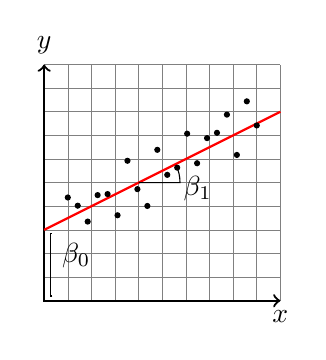
\begin{tikzpicture}[scale=0.15]
\draw[step=2, gray, very thin] (-10,-10) grid (10,10); % background grid
\draw[thick, <->] (-10,10) node[anchor=south] {$y$} -- (-10,-10) -- (10,-10) node[anchor=north] {$x$}; %axis
\draw[red, thick] plot [domain=-10:10] (\x,{1 + 0.5 * \x}); % regression line
\draw plot [only marks, mark=*, mark size=6, domain=-8:8, samples=20] (\x,{rnd * 5 - 1.5 + 0.5 * \x}); % data points
\draw (-9.3,-9.6) -- (-9.5,-9.6) -- (-9.5,-4.3) -- (-9.3, -4.3) node[anchor=north west] {$\beta_0$}; % beta0
\draw (-2,0) -- (1.5,0) arc (0:25:3.5); % beta1 arc
\draw (3,-0.5) node {$\beta_1$}; % beta1
\end{tikzpicture}

\columnbreak

Ecuación:\\ $y_i = \beta_0 + \beta_1 x_{1i} + u_i$

\vspace*{1mm}

Estimación:\\ $\hat{y}_i = \hat{\beta}_0 + \hat{\beta}_1 x_{1i}$

\vspace*{1mm}

Donde: \\ $\hat{\beta}_0 = \overline{y} - \hat{\beta}_1 \overline{x}$ \\ $\hat{\beta}_1 = \frac{Cov(y, x)}{Var(x)}$

\end{multicols}

\subsection*{Modelo de regresión múltiple}

\setlength{\multicolsep}{0pt} % reduce vertical spacing betwen subsection and multicols
\setlength{\columnsep}{-40pt} % reduce spacing between columns
\begin{multicols}{2} % set columns to 2

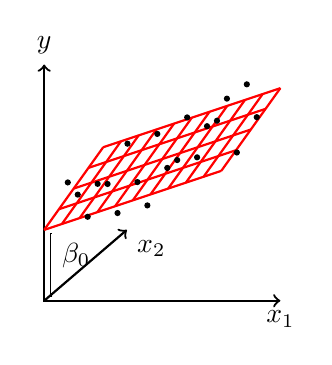
\begin{tikzpicture}[scale=0.15]
\draw[thick, ->] (-10,-10) -- (-3,-4) node[anchor=north west] {$x_2$}; % x2 axis
\draw[thick, <->] (-10,10) node[anchor=south] {$y$} -- (-10,-10) -- (10,-10) node[anchor=north] {$x_1$}; % y and x1 axis
% regression grid
\draw[red, thick] (-10,-4) -- (-5,3);
\draw[red, thick] (-8.5, -3.5) -- (-3.5,3.5);
\draw[red, thick] (-7, -3) -- (-2,4);
\draw[red, thick] (-5.5, -2.5) -- (-0.5,4.5);
\draw[red, thick] (-4, -2) -- (1,5);
\draw[red, thick] (-2.5, -1.5) -- (2.5,5.5);
\draw[red, thick] (-1, -1) -- (4,6);
\draw[red, thick] (0.5, -0.5) -- (5.5,6.5);
\draw[red, thick] (2, 0) -- (7,7);
\draw[red, thick] (3.5, 0.5) -- (8.5,7.5);
\draw[red, thick] (5, 1) -- (10,8);
\draw[red, thick] (-10, -4) -- (5, 1);
\draw[red, thick] (-8.75, -2.25) -- (6.25,2.75);
\draw[red, thick] (-7.5, -0.5) -- (7.5,4.5);
\draw[red, thick] (-6.25, 1.25) -- (8.75,6.25);
\draw[red, thick] (-5,3) -- (10,8);
\draw plot [only marks, mark=*, mark size=6, domain=-8:8, samples=20] (\x,{rnd * 6.5 - 1.5 + 0.5 * \x}); % data points
\draw (-9.3,-9.6) -- (-9.5,-9.6) -- (-9.5,-4.3) -- (-9.3, -4.3) node[anchor=north west] {$\beta_0$}; % beta0
\end{tikzpicture}

\columnbreak

Ecuación: \\ $y_i = \beta_0 + \beta_1 x_{1i} + ... + \beta_k x_{ki} + u_i$

\vspace*{1mm}

Estimación: \\ $\hat{y}_i = \hat{\beta}_0 + \hat{\beta}_1 x_{1i} + ... + \hat{\beta}_k x_{ki}$

\vspace*{1mm}

Donde: \\ $\hat{\beta}_0 = \overline{y} - \hat{\beta}_1 \overline{x}_1 - ... - \hat{\beta}_k \overline{x}_k$ \\ $\hat{\beta}_j = \frac{Cov(y, \text{residualizado } x_j)}{Var(\text{residualizado } x_j)}$

\vspace*{1mm}

Matriz: $\hat{\beta} = (X^T X)^{-1} (X^T y)$

\end{multicols}

\subsection*{Interpretación de coeficientes}

\scalebox{0.872}{ % scale the table to fit in the column
\begin{tabular}{ c c c c }
	Modelo & Depend. & Independ. & Interpretación $\beta_1$ \\
	\hline
	Nivel-nivel & $y$ & $x$ & $\Delta y = \beta_1 \Delta x$ \\ 
	Nivel-log & $y$ & $log(x)$ & $\Delta y = (\beta_1/100) \% \Delta x$ \\  
	Log-nivel & $log(y)$ & $x$ & $\% \Delta y = (100 \beta_1) \Delta x$ \\
	Log-log & $log(y)$ & $log(x)$ & $\% \Delta y = \beta_1 \% \Delta x$ \\
	Cuadrático & $y$ & $x + x^2$ & $\Delta y = (\beta_1 + 2 \beta_2 x) \Delta x$ \\
\end{tabular}
}

\subsection*{Medidas de error}

Suma de Resid. Cuad.: \hfill $SRC = \sum_{i=1}^n \hat{u}_i^2 = \sum_{i=1}^n (y_i - \hat{y}_i)^2$

\vspace*{0.5mm}

Suma Expl. de Cuad.: \hfill $SEC = \sum_{i=1}^n (\hat{y}_i - \overline{y})^2$

\vspace*{0.5mm}

Suma Tot. de Cuad.: \hfill $STC = SEC + SRC = \sum_{i=1}^n (y_i - \overline{y})^2$

\vspace*{0.5mm}

Error Estándar de la Regresión: \hfill $\hat{\sigma} = \sqrt{\frac{SSR}{n-k-1}}$

\vspace*{0.5mm}

Error Estándar de los $\hat{\beta}$'s: \hfill $ee(\hat{\beta}) = \hat{\sigma} \sqrt{(X^T X)^{-1}}$

\vspace*{0.5mm}

Raíz Cuadrada del Error Cuadrático Medio: \hfill $\sqrt{\frac{\sum_{i=1}^n (\hat{u}_i - \overline{u})^2}{n}}$

\vspace*{0.5mm}

Error Medio Absoluto: \hfill $\frac{\sum_{i=1}^n |\hat{u}_i|}{n}$

\vspace*{0.5mm}

Porcentaje Medio de Error: \hfill $\frac{\sum_{i=1}^n |\hat{u}_i / y_i|}{n} \times 100$

\columnbreak

\section*{R-cuadrado}

Es una \textbf{medida de la bondad del ajuste}, cómo la regresión se ajusta a los datos:

\begin{center}
$R^2 = \frac{SEC}{STC} = 1 - \frac{SRC}{STC}$
\end{center}

\begin{itemize}[leftmargin=*]
\item Mide el \textbf{porcentaje de variación en $y$ que es linealmente explicado por variaciones de las $x$'s}.
\item Toma valores \textbf{entre 0} (no hay explicación lineal de las variaciones de $y$) \textbf{y 1} (explicación total de las variaciones de $y$).
\end{itemize}

Cuando el número de regresores incrementa, el valor del r-cuadrado también lo hace, independientemente de si las nuevas variables son relevantes o no. Para resolver este problema, existe un \textbf{r-cuadrado corregido por grados de libertad} (o r-cuadrado ajustado):

\begin{center}
$\overline{R}^2 = 1 - \frac{n-1}{n-k-1} \frac{SRC}{STC} = 1 - \frac{n-1}{n-k-1} (1-R^2)$
\end{center}

Para muestras grandes: $\overline{R}^2 \approx R^2$

\section*{Contrastes de hipótesis}
\subsection*{Base de los contrastes de hipótesis}

Un contraste de hipótesis es una regla diseñada para, a partir de una muestra, \textbf{explicar si existe evidencia para rechazar (o no) una hipótesis} sobre uno o más parámetros poblacionales.

Elementos de un contraste de hipótesis:

\begin{itemize}[leftmargin=*]
\item \textbf{Hipótesis nula ($H_0$)} - es la hipótesis a ser probada.
\item \textbf{Hipótesis alternativa ($H_1$)} - el la hipótesis que no puede rechazarse si la hipótesis nula es rechazada.
\item \textbf{Estadístico de contraste}: es una variable aleatoria cuya distribución de probabilidad es conocida bajo la hipótesis nula y está tabulada.
\item \textbf{Nivel de significación ($\alpha$)} - es la probabilidad de rechazar la hipótesis nula siendo cierta (error Tipo I). Es elegido por quien conduce el contraste. Usualmente es 0.10, 0.05, 0.01 ó 0.001.
\item \textbf{Valor crítico} - es el valor contra el cual se compara el estadístico de contraste para determinar si se rechaza o no la hipótesis nula.
\item \textbf{p-valor} - es el nivel de significación máximo por el cual la hipótesis nula no puede ser rechazada ($H_0$).
\end{itemize}

\textbf{Regla general}: si el p-valor es menor que $\alpha$, existe evidencia para rechazar la hipótesis nula a ese determinado $\alpha$ (existe evidencia para aceptar la hipótesis alternativa).

\subsection*{Contrastes individuales}

Prueba si un parámetro es significativamente diferente de un cierto valor, $\theta$.

\begin{itemize}[leftmargin=*]
\item $H_0: \beta_j = \theta$
\item $H_1: \beta_j \neq \theta$
\end{itemize}

Bajo $H_0$:

\begin{center}
$t = \frac{\hat{\beta}_j - \theta}{ee(\hat{\beta}_j)} \sim t_{n-k-1, \alpha/2}$
\end{center}

Si $\mid t \mid > t_{n-k-1, \alpha/2}$, existe evidencia para rechazar la hipótesis nula.

\textbf{Contraste de significación individual} - prueba si un parámetro es \textbf{significativamente distinto de cero}.

\begin{itemize}[leftmargin=*]
\item $H_0: \beta_j = 0$
\item $H_1: \beta_j \neq 0$
\end{itemize}

Bajo $H_0$:

\begin{center}
$t = \frac{\hat{\beta}_j}{ee(\hat{\beta}_j)} \sim t_{n-k-1, \alpha/2}$
\end{center}

Si $\mid t \mid > t_{n-k-1, \alpha/2}$, existe evidencia para rechazar la hipótesis nula.

\subsection*{Contraste F}

Prueba simultáneamente múltiples hipótesis (lineales) sobre los parámetros. Hace uso de un modelo no restringido y uno restringido:

\begin{itemize}[leftmargin=*]
\item \textbf{Modelo no restringido} - es el modelo donde se quiere probar la hipótesis.
\item \textbf{Modelo restringido} - es el modelo donde se ha impuesto la hipótesis que se quiere probar.
\end{itemize}

Entonces, viendo los errores, hay:

\begin{itemize}[leftmargin=*]
\item \textbf{$\sum_{i=1}^n \hat{u}_{nr}^2$} - es la Suma de Resid. Cuadrados del modelo no restringido ($SRC_{nr}$).
\item \textbf{$\sum_{i=1}^n \hat{u}_r^2$} - es la Suma de Resid. Cuadrados del modelo restringido ($SRC_r$).
\end{itemize}

Bajo $H_0$:

\begin{center}
$F = \frac{SRC_r - SRC_{nr}}{SRC_{nr}} \frac{(n-k_{nr}-1)}{q} \sim F_{q, n-k_{nr}-1}$
\end{center}

Donde $k_{nr}$ es el número de parámetros del modelo no restringido y $q$ es el número de hipótesis lineales a probar.

Si $F_{q, n-k_{nr}-1} < F$, existe evidencia para rechazar la hipótesis nula.

\textbf{Contraste de significación global} - prueba si todos los parametros asociados a $x$'s son simultáneamente iguales a cero.

$H_0: \beta_1 = \beta_2 = ... = \beta_k = 0$

$H_1: \beta_1 \neq 0$ and/or $\beta_2 \neq 0 ...$ and/or $\beta_k \neq 0$

Si $F_{k, n-k_{nr}-1} < F$, existe evidencia para rechazar la hipótesis nula.

\section*{Intervalos de confianza}

Los intervalos de confianza al nivel de confianza ($1 - \alpha$), se pueden calcular:

\begin{center}
$\hat{\beta}_j \mp t_{n-k-1, \alpha/2} ee(\hat{\beta}_j)$
\end{center}

\section*{Variables ficticias y cambio estructural}

Las variables ficticias (o binarias) son usadas para recoger información cualitativa: sexo, estado civil, país, etc.

\begin{itemize}[leftmargin=*]
\item Toman \textbf{el valor de 1 en una categoría dada, y 0 en el resto}.
\item Se usan para analizar y modelizar \textbf{cambios estructurales} en los parámetros del modelo.
\end{itemize}

Si una variable cualitativa tiene $m$ categorías, sólo hay que incluir ($m-1$) variables ficticias en el modelo.

\subsection*{Cambio estructural}

El cambio estructural se refiere a los cambios en los valores de los parámetros del modelo producidos por el efecto de diferentes sub-poblaciones. El cambio estructural se puede incluir en el modelo a través de variables ficticias.

La posición de las variables ficticias es importante:
\begin{itemize}[leftmargin=*]
\item \textbf{En el intercepto ($\beta_0$)} - representa la diferencia media entre los valores producidos por el cambio estructural.
\item \textbf{En los parámetros que determinan la pendiente de la línea de regresión ($\beta_j$)} - representa la diferencia en el efecto (pendiente) entre los valores producidos por el cambio estructural.
\end{itemize}

\textbf{El contraste de Chow para cambio estructural} - cuando se quiere analizar la existencia de cambio estructural en todos los parámetros del modelo, es común hacer uso de una expresión particular del contraste F, conocido como el contraste de Chow, donde la hipótesis nula es: $H_0: \text{No hay cambio estructural}$

\section*{Predicciones}

Dos tipos de predicciones:

\begin{itemize}[leftmargin=*]
\item Del valor medio de $y$ para un valor específico de $x$.
\item De un valor individual de $y$ para un valor específico de $x$.
\end{itemize}

Si los valores de las variables ($x$) se aproximan al valor medio ($\overline{x}$), la amplitud del intervalo de confianza de la predicción será menor. 

\columnbreak

\section*{Multicolinealidad}

\begin{itemize}[leftmargin=*]
\item \textbf{Multicolinealidad perfecta} - hay variables independientes que son constantes y/o hay una relación lineal exacta entre variables independientes. Es el \textbf{incumplimiento del tercer (3) supuesto del modelo}.
\item \textbf{Multicolinealidad aproximada} - hay variables independientes que son aproximadamente constantes y/o hay una relación lineal aproximada entre variables independientes. \textbf{No implica el incumplimiento de algún supuesto del modelo}, pero tiene un efecto en MCO.
\end{itemize}

\subsection*{Consecuencias}

\begin{itemize}[leftmargin=*]
\item \textbf{Multicolinealidad perfecta} - el sistema de ecuaciones de MCO no puede resolverse (infinitas soluciones).
\item \textbf{Multicolinealidad aproximada}
\begin{itemize}[leftmargin=*]
\item Pequeñas variaciones en la muestra producen grandes variaciones en las estimaciones de MCO.
\item La varianza de los estimadores MCO de las $x$'s que son colineales incrementa, la inferencia de los parámetros es afectada (intervalo de confianza grande).
\end{itemize}
\end{itemize}

\subsection*{Detección}

\begin{itemize}[leftmargin=*]
\item \textbf{Análisis de correlación} - buscar altas correlaciones (mayores a 0.7) entre variables independientes.
\item \textbf{Factor de Inflación de la Varianza (FIV o VIF)} - indica el incremento en $Var(\hat{\beta}_j)$ debido a la multicolinealidad.
\begin{center}
$VIF(\hat{\beta}_j) = \frac{1}{1-R_j^2}$
\end{center}
Donde $R^2_j$ denota el r-cuadrado de una regresión entre $x_j$ y todas las otras $x$'s. 
\begin{itemize}[leftmargin=*]
\item Valores entre 4 y 10 sugieren que es recomendable analizar en mayor profundidad si pueden existir problemas de multicolinealidad.
\item Valores por encima de 10 indican que existen problemas de multicolinealidad.
\end{itemize}
\end{itemize}

Una característica típica de la multicolinealidad es que los coeficientes de regresión del modelo no son individualmente significativos (por las altas varianzas), pero sí que son conjuntamente significativos.

\subsection*{Corrección}

\begin{itemize}[leftmargin=*]
\item Eliminar una de las variables colineales.
\item Realizar análisis factorial(u otra técnica de reducción de dimensiones) en las vairables colineales.
\item Interpretar los coeficientes con multicolinealidad de manera conjunta.
\end{itemize}

\columnbreak

\section*{Heterocedasticidad}

Los residuos $u_i$ de la función de regresión poblacional no tienen una varianza constante $\sigma^2$:

\begin{center}
$Var(u|x) = Var(y|x) \neq \sigma^2$
\end{center}

Es el \textbf{incumplimiento del quinto (5) supuesto del modelo}.

\subsection*{Consecuencias}

\begin{itemize}[leftmargin=*]
\item Estimadores MCO son insesgados.
\item Estimadores MCO son consistentes.
\item MCO ya \textbf{no es eficiente}, pero sigue siendo ELI (Estimador Lineal Insesgado).
\item La \textbf{estimación de la varianza de los estimadores es sesgada}: la construcción de intervalos de confianza y contraste de hipótesis no son fiables.
\end{itemize}

\subsection*{Detección}

\begin{itemize}[leftmargin=*]
\setlength{\multicolsep}{0pt} % reduce vertical spacing betwen subsection and multicols
\setlength{\columnsep}{20pt} % increment spacing between columns
\begin{multicols}{3} % set columns to 3
\item \textbf{Gráficos} - buscar patrones de dispersión en gráficos $x$ vs. $u$ ó $x$ vs. $y$.

\columnbreak

\vspace*{-23pt}

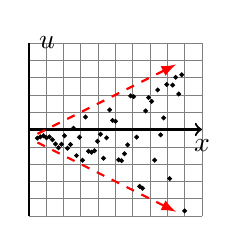
\begin{tikzpicture}[scale=0.11]
\draw[step=2, gray, very thin] (-10,-10) grid (10,10); % grid
\draw[thick,->] (-10,0) -- (10,0) node[anchor=north] {$x$}; % x axis
\draw[thick,-] (-10,-10) -- (-10,10) node[anchor=west] {$u$}; % u axis
\draw plot [only marks, mark=*, mark size=6, domain=0:17, samples=50] ({\x - 9},{-0.5 * rand * \x - 1}); % data points
\draw[thick, dashed, red, -latex] plot [domain=1:17] ({\x - 10},{-0.5 * \x - 1}); % lower red arrow
\draw[thick, dashed, red, -latex] plot [domain=1:17] ({\x - 10},{0.5 * \x - 1}); % upper red arrow
\end{tikzpicture}

\columnbreak

\vspace*{-24pt}

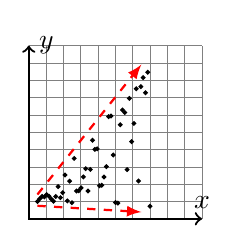
\begin{tikzpicture}[scale=0.11]
\draw[step=2, gray, very thin] (-10,-10) grid (10,10); % grid
\draw[thick,<->] (-10,10) node[anchor=west] {$y$} -- (-10,-10) -- (10,-10) node[anchor=south] {$x$}; % axis
\draw plot [only marks, mark=*, mark size=6, domain=0:13, samples=50] ({\x -9},{(-0.65 * rand * \x) + 0.6 * \x - 8}); % data points
\draw[thick, dashed, red, -latex] plot [domain=0:12] ({\x - 9},{-0.06 * \x - 8.5}); % lower red arrow
\draw[thick, dashed, red, -latex] plot [domain=0:12] ({\x -9},{1.25 * \x - 7.2}); % upper red arrow
\end{tikzpicture}

\end{multicols}

\item \textbf{Test formales} - White, Bartlett, Breusch-Pagan, etc. Comúnmente, la hipótesis nula: $H_0 = \text{Homocedasticidad}$
\end{itemize}

\subsection*{Corrección}

\begin{itemize}[leftmargin=*]
\item Usar MCO con un estimador de la matriz de varianzas-covarianzas robusto a la heterocedasticidad, por ejemplo, la propuesta de White.
\item Si la estructura de la varianza es conocida, usar Mínimos Cuadrados Ponderados (MCP) o Mínimos Cuadrados Generalizados (MCG).
\item Si la estructura de la varianza es desconocida, hacer uso de Mínimos Curadrados Ponderados Factibles (MCPF), que estima una posible varianza, divide las variables del modelo entre ella y entonces aplica MCO.
\item Hacer suposiciones sobre la posible varianza:
\begin{itemize}[leftmargin=*]
\item Suponiendo que $\sigma_i^2$ es proporcional a $x_i$, dividir las variables del modelo entre la raíz cuadrada de $x_i$ y aplicar MCO.
\item Suponiendo que $\sigma_i^2$ es proporcional a $x_i^2$, dividir las variables del modelo entre $x_i$ y aplicar MCO.
\end{itemize}
\item Nueva especificación del modelo, por ejemplo, transformación logarítmica.
\end{itemize}

\columnbreak

\section*{Autocorrelación}

El residuo de cualquier observación, $u_t$, está correlacionado con el residuo de cualquier otra observación. Las observaciones no son independientes.

\begin{center}
$Corr(u_t, u_s | x) \neq 0$ para cualquier $t \neq s$
\end{center}

El contexto ``natural" de este fenómeno son las series temporales. Es el \textbf{incumplimiento del sexto (6) supuesto del modelo}.

\subsection*{Consequences}

\begin{itemize}[leftmargin=*]
\item Estimadores MCO son insesgados.
\item Estimadores MCO son consistentes.
\item MCO ya \textbf{no es eficiente}, pero sigue siendo ELI (Estimador Lineal Insesgado).
\item La \textbf{estimación de la varianza de los estimadores es sesgada}: la construcción de intervalos de confianza y contraste de hipótesis no son fiables.
\end{itemize}

\subsection*{Detection}

\begin{itemize}[leftmargin=*]
\item \textbf{Gráficos} - buscar patrones de dispersión en gráficos $u_{t-1}$ vs. $u_t$ o hacer uso del correlograma.

\setlength{\multicolsep}{0pt} % reduce vertical spacing betwen subsection and multicols
\setlength{\columnsep}{6pt} % increment spacing between columns
\begin{multicols}{3} % set columns to 3

\begin{center}
\textbf{\footnotesize AR}
\end{center}

\vspace{2.0pt}

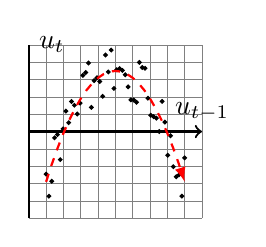
\begin{tikzpicture}[scale=0.11]
\draw[step=2, gray, very thin] (-10,-10) grid (10,10); % grid
\draw[thick,->] (-10,0) -- (10,0) node[anchor=south] {$u_{t-1}$}; % ut-1 axis
\draw[thick,-] (-10,-10) -- (-10,10) node[anchor=west] {$u_t$}; % ut axis
\draw plot [only marks, mark=*, mark size=6, domain=-8:8, samples=50] (\x,{rnd * 6 + (-2 * (\x)^2 + 40) * 0.1}); % data points
\draw[thick, dashed, red, -latex] plot [domain=-8:8] (\x,{3 + (-2 * (\x)^2 + 40) * 0.1}); % red arrow
\end{tikzpicture}

\columnbreak

\begin{center}
\textbf{\footnotesize AR(+)}
\end{center}

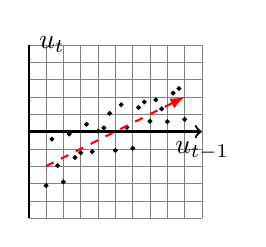
\begin{tikzpicture}[scale=0.11]
\draw[step=2, gray, very thin] (-10,-10) grid (10,10); % grid
\draw[thick,->] (-10,0) -- (10,0) node[anchor=north] {$ u_{t-1}$}; % ut-1 axis
\draw[thick,-] (-10,-10) -- (-10,10) node[anchor=west] {$u_t$}; % ut axis
\draw plot [only marks, mark=*, mark size=6, domain=-8:8, samples=25] (\x,{rnd * 6 + 0.5 * \x - 3}); % data points
\draw[thick, dashed, red, -latex] plot [domain=-8:8] (\x,{3 + 0.5 * \x - 3}); % red arrow
\end{tikzpicture}

\columnbreak

\begin{center}
\textbf{\footnotesize AR(-)}
\end{center}

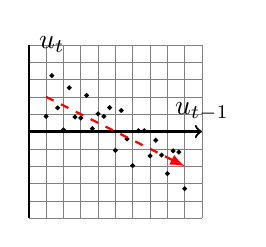
\begin{tikzpicture}[scale=0.11]
\draw[step=2, gray, very thin] (-10,-10) grid (10,10); % grid
\draw[thick,->] (-10,0) -- (10,0) node[anchor=south] {$u_{t-1}$}; % ut-1 axis
\draw[thick,-] (-10,-10) -- (-10,10) node[anchor=west] {$u_t$}; % ut axis
\draw plot [only marks, mark=*, mark size=6, domain=-8:8, samples=25] (\x,{rnd * 6 - 0.5 * \x - 3}); % data points
\draw[thick, dashed, red, -latex] plot [domain=-8:8] (\x,{3 - 0.5 * \x - 3}); % red arrow
\end{tikzpicture}

\end{multicols}

\item \textbf{Test formales} - Durbin-Watson, Breusch-Godfrey, etc. Comúnmente, la hipótesis nula: $H_0: \text{No autocorrelación}$

\end{itemize}

\subsection*{Corrección}

\begin{itemize}[leftmargin=*]
\item Usar MCO con un estimador de la matriz de varianzas-covarianzas robusto a la autocorrelación, por ejemplo, la propuesta de Newey-West.
\item Usar Mínimos Cuadrados Generalizados. Suponiendo $y_t = \beta_0 + \beta_1 x_t + u_t$, con $u_t = \rho u_{t-1} + \varepsilon_t$, donde $|\rho| < 1$ y $\varepsilon_t$ es ruido blanco.
\begin{itemize}[leftmargin=*]
\item Si $\rho$ es conocido, crear un modelo cuasi-diferenciado donde $u_t$ es ruido blanco y estimarlo por MCO.
\item Si $\rho$ es desconocido, estimarlo -por ejemplo- por el método de Cochrane-Orcutt, crear un modelo cuasi-diferenciado donde $u_t$ es ruido blanco y estimarlo por MCO.
\end{itemize}
\end{itemize}

\end{multicols}
\end{document}